\documentclass{article}
%=======================================================
%                      Dependencies
%=======================================================
\usepackage{graphicx}
\usepackage{multicol}
\usepackage{amsmath}
\usepackage{pgfplots}
\usepackage{tabularx}
\usepackage{wrapfig}

\begin{document}
%=======================================================
%                      Front Page
%=======================================================
\begin{titlepage}
  {
\includegraphics[width=0.3\textwidth]{multimedia/ESCOM-Logo.png}}
  \hfill
  {\includegraphics[width=0.15\textwidth]{multimedia/Logo_Instituto_Politécnico_Nacional.png}\par}
  \vspace{1cm}
  \centering
  {\bfseries\LARGE  INSTITUTO POLIT\'ECNICO NACIONAL\par}
  \vspace{1cm}
  {\scshape\LARGE Escuela Superior de C\'omputo\par}
  \vspace{1cm}
  {\scshape\Huge Unidad 1: La integral definida y sus aplicaciones \par}
  \vspace{2cm}
  {\itshape\Large Zarate Cardenas Alejandro\par}
  \vfill
  {\Large Autores:\par}
  {\Large Campos Zeron Salvador\par}
  {\Large Díaz González Lizeth\par}
  {\Large Girón Flores Carlos Alberto\par}
  {\Large Hernández García Jaime Gabriel\par}
  {\Large Izoteco Zacarias Pedro Uriel\par}
  {\Large S\'anchez Ortega Gabriel\par}
  \vfill
  {\Large 10 de Marzo 2023 \par}
\end{titlepage}

%=====================================================
%                         Content
%=====================================================
\renewcommand*\contentsname{Índice}
\tableofcontents
\newpage
\section{Introducción}

La integral definida es uno de los conceptos fundamentales en el cálculo, una rama de las matemáticas que estudia el cambio y la variación. La integral definida es una operación matemática que permite calcular el valor de una función en un intervalo específico. A diferencia de la integral indefinida, que devuelve una familia de funciones, la integral definida da como resultado un número único.

La integral definida tiene múltiples aplicaciones en diversas áreas de la ciencia, la ingeniería y la economía. En física, la integral definida se utiliza para calcular la energía cinética y potencial, la velocidad y la aceleración de un objeto en movimiento. En ingeniería, se utiliza para diseñar puentes, carreteras y edificios, y para optimizar procesos industriales. En economía, la integral definida se utiliza para calcular el valor presente de una inversión o el flujo de caja de una empresa. En biología, se utiliza para modelar el crecimiento de poblaciones y la distribución de especies en un ecosistema.

Para calcular una integral definida, se divide el intervalo en pequeñas secciones llamadas subintervalos y se aproxima el valor de la función en cada uno de ellos. Luego, se suman los resultados de cada subintervalo para obtener una aproximación del valor de la integral. A medida que se dividen los subintervalos en secciones más pequeñas, la aproximación se vuelve más precisa.

En resumen, la integral definida es una herramienta matemática poderosa con innumerables aplicaciones prácticas en diversas áreas. Es una herramienta fundamental en el cálculo y se utiliza para calcular el área bajo una curva, la longitud de una curva y el volumen de un sólido de revolución, entre otras cosas. Su importancia en la ciencia y la ingeniería es crucial para el avance y desarrollo de la tecnología moderna.
\subsection{Lo que revisamos}
A lo largo de este documento se podra ver la resolucion de los problemas propuestos en el libro anteriormente mencionado aclarando que dichos problemas fueron divididos por equipo tocandole al "Equipo Capibara" los problemas impares(5,17,29,41,53) de las paginas: 293-295, 303-305, 313-314, 331-332, 430-432
\section{Problemario 1: 293-295}

\subsection{Problema 5}
Desarrolle la suma indicada:
\begin{equation}\label{eq_5.1}
  \sum_{k=1}^{10}\frac{(-1)^k}{2k+5}
\end{equation}
Donde si hacemos a sumatoria dada por la ecuacion \ref{eq_5.1} tenemos:
\begin{equation}\label{eq_5.2}
  \begin{split}
    \frac{(-1)^1}{2(1)+5}+\frac{(-1)^2}{2(2)+5}+\frac{(-1)^3}{2(3)+5}+\frac{(-1)^4}{2(4)+5}+\frac{(-1)^5}{2(5)+5}+\\\frac{(-1)^6}{2(6)+5}+\frac{(-1)^7}{2(7)+5}+\frac{(-1)^8}{2(8)+5}+\frac{(-1)^9}{2(9)+5}+\frac{(-1)^{10}}{2(10)+5}
  \end{split}
\end{equation}
Realizando las respectivas operaciones en \ref{eq_5.2}
\begin{equation}\label{eq_5.3}
  -\frac{1}{7}+\frac{1}{9}-\frac{1}{11}+\frac{1}{13}-\frac{1}{15}+\frac{1}{17}-\frac{1}{19}+\frac{1}{21}-\frac{1}{23}+\frac{1}{25} = -0.062065975\dots
\end{equation}
Teniendo asi que el resultado esta dado en la ecuacion \ref{eq_5.4}, es decir, la que esta a continuacion:
\begin{equation}\label{eq_5.4}
  \sum_{k=1}^{10}\frac{(-1)^k}{2k+5} = -0.062065975\dots
\end{equation}
\subsection{Problema 17}
Escriba en notación sigma la suma dada
\setcounter{equation}{0}
\begin{equation}\label{eq_17.1}
  6+6+6+6+6+6+6+6
\end{equation}
Contando el numero de veces que aparce el 6 en la suma \ref{eq_17.1} tenemos que k(contador) toma valores de 1 a 8 dejandonos con la siguiente expresion:
\begin{equation}\label{eq_17.2}
  \sum_{k=1}^{8}6
\end{equation}
\setcounter{equation}{0}
\subsection{Problema 29}
Utilizando lo siguiente:
\begin{equation} \label{prop_area}
  A = \lim_{n\to\infty} \sum_{k=1}^{n} f\left(a+k\frac{b-a}{n}\right)* \frac{b-a}{n}
\end{equation}
Y los siguientes teoremas:
\begin{align*}
  \sum_{k=1}^{n} c & = nc & \sum_{k=1}^{n} k & = \frac{n(n+1)}{2} \\ \sum_{k=1}^{n} k^2 &= \frac{n(n+1)(2n+1)}{6} & \sum_{k=1}^{n} k^3 &= \frac{n^2(n+1)^2}{4}
\end{align*}
Con la propiedad dada en la ecuacion \ref{prop_area} y los teoremas dados anteriormente calcule el area bajo la funcion siguiente:
\begin{equation}
  f(x) = x, [0,6]
\end{equation}
Con dicha informacion podemos decir que:
\begin{align*}
  a & = 0 & b & = 6
\end{align*}
Entonces:
\begin{equation}
  A = \lim_{n\to\infty} \sum_{k=1}^{n} f\left(0+k\frac{6-0}{n}\right)* \frac{6-0}{n}
\end{equation}
Desarrollando:
\begin{align*}
  A = \lim_{n\to\infty} \sum_{k=1}^{n} f\left(k\frac{6}{n}\right)* \frac{6}{n} =\dots \\\dots = \lim_{n\to\infty} \sum_{k=1}^{n} \left(\frac{36k}{n^2}\right)=\lim_{n\to\infty}\left[\frac{36}{n^2} \sum_{k=1}^{n} k\right]=\dots \\ \dots = \lim_{n\to\infty}\left[\frac{36}{n^2} *\frac{n(n+1)}{2}\right]=\lim_{n\to\infty} \left[18*\frac{n(n+1)}{n^2}\right]=\dots \\ \dots = 18\lim_{n\to\infty} \left[\frac{n+1}{n}\right]= 18*1=18
\end{align*}
Por lo tanto $A = 18$
\subsection{Problema 41}
Utilizando los teoremas y la definicion del problema anteriror resuelva lo siguiente:
\begin{equation*}
  f(x) = \left\{
  \begin{array}{lcc}
    2,   & si & 0\leq x < 1     \\
    x+1, & si & 1 \leq x \leq 4
  \end{array}
  \right.
\end{equation*}
Entonces podemos decir que el area esta dada por:
\begin{equation}
  A = \int_{0}^{1} f(x)dx + \int_{1}^{5} f(x)dx
\end{equation}
Gracias a esta suma podemos trabajar por separado los dos trozos de la funcion. Asi facilitando s manipulacion.
Para el segmento de $\int_{0}^{1}f(x)dx$ la funcion esta evaluada en 2. Por lo cual el area esta dada por un valor constante y para este caso debemos agregar una propiedad:
\begin{equation}
  \int_{a}^{b}kdx = k\int_{a}^{b}dx = k(b-a)
\end{equation}
Sustituyendo:
\begin{equation}
  A_1=\int_{0}^{1}2dx = 2\int_{0}^{1}dx = 2(1-0)=2
\end{equation}
Trabajando con la segunda parte tenemos:
\begin{equation}
  A_2 = \int_{1}^{4} f(x)dx = \int_{1}^{4}xdx + \int_{1}^{4}1dx
\end{equation}
Trabajando por partes:
\begin{align*}
  i) \int_{1}^{4}xdx                                                                            & =\dots & ii) 1\int_{1}^{4}dx & = \dots \\ \dots=\lim_{n\to\infty} \sum_{k=1}^{n}\left[1+\frac{3k}{n}\right]\cdot\frac{3}{n}&=\dots & \dots = 1(4-1)&=3 \\
  \dots=\lim_{n\to\infty} \sum_{k=1}^{n}\left[\frac{3}{n}+\frac{9k}{n^2}\right]\cdot\frac{3}{n} & =\dots                                 \\ \dots = \lim_{n\to\infty}\left[3+\frac{9}{n^2}\cdot\frac{n(n+1)}{2}\right] = \dots \\ \dots=\lim_{n\to\infty}\left[3+\frac{9}{2}\cdot\frac{n+1}{n}\right]= 3+\frac{9}{2} = \frac{15}{2}
\end{align*}
Ya que se tienen las integrales por partes tenemos lo siguiente:
\begin{equation}
  A_2 = \int_{1}^{4}xdx = \frac{15}{2} + 3 = \frac{21}{2}
\end{equation}
Para terminar realizamos la suma entre \(A_1\) y \(A_2\) para obtener \(A_T\):
\begin{equation}
  A_T = \int_{0}^{4} f(x)dx = A_1 + A_2 = \frac{21}{2} + 2 = \frac{25}{2}
\end{equation}
\subsection{Problema 53}
Despeje \(\bar{x}\) de :
\begin{equation}
  \sum_{k=1}^{n}(x_k-\bar{x})^2 = 0
\end{equation}
Desarrollando:
\begin{align*}
  \sum_{k=1}^{n}x^2_k - 2x_k\bar{x} + \bar{x}^2=0 \\ \sum_{k=1}^{n}x^2_k -\sum_{k=1}^{n} 2x_k\bar{x} + \sum_{k=1}^{n} \bar{x}^2 = 0 \\ \sum_{k=1}^{n} x^2_k -2\bar{x}\sum_{k=1}^{n}x_k + \bar{x}^2=0 \\ \bar{x}^2-2\bar{x}\sum_{k=1}^{n}x_k = -\sum_{k=1}^{n} x^2_k \\ \bar{x}^2-2\bar{x}\sum_{k=1}^{n}x_k + \left(\sum_{k=1}^{n} x_k\right)^2 = \left(\sum_{k=1}^{n} x_k\right)^2 -\sum_{k=1}^{n} x^2_k \\ \left(\bar{x} + \sum_{k=1}^{n} x_k \right)^2 = \left(\sum_{k=1}^{n} x_k\right)^2 -\sum_{k=1}^{n} x^2_k \\ \bar{x} + \sum_{k=1}^{n} x_k = \sqrt{\left(\sum_{k=1}^{n} x_k\right)^2 -\sum_{k=1}^{n} x^2_k} \\ \bar{x} = \sqrt{\left(\sum_{k=1}^{n} x_k\right)^2 -\sum_{k=1}^{n} x^2_k} - \sum_{k=1}^{n} x_k
\end{align*}
\subsection{Conclusión}
En conclusión, las sumas de Riemann son una técnica matemática utilizada para aproximar el valor de una integral definida. Esta técnica se basa en dividir el intervalo de integración en subintervalos y aproximar el valor de la función en cada uno de ellos. A medida que se divide el intervalo en secciones más pequeñas, la aproximación se vuelve más precisa. Las sumas de Riemann son una herramienta esencial en el cálculo y tienen aplicaciones en diversas áreas, como la física, la ingeniería y la economía. Además, son la base para el desarrollo del cálculo integral, una rama fundamental de las matemáticas.
\section{Problemario 2: 303-305}
\subsection{Problema 5}
Sea una funcion \(f(x)\) definida por: \(f(x) = sin(x)\) calcule el area dada por el intervalo cerrado: \([0,2\pi]\) considerando los siguientes subintervalos: $$x_0 = 0; x_1 = \pi; x_2 = \frac{3\pi}{2}; x_3 = 2\pi$$ y: $$x_1^*=\frac{\pi}{2}; x_2^*=\frac{7\pi}{6}; x_3^* = \frac{7\pi}{4}$$
Como ya sabemos el area se calcula con: $$\sum_{k=1}^{n}f(x^*_k) \bigtriangleup  x_k$$
Por lo que desarrollando tenemos:
\begin{align*}
  \sum_{k=1}^{3}f(x^*_k) \bigtriangleup  x_k                      &  & = &  & f(x_1^*)\bigtriangleup x_1 + f(x_2^*)\bigtriangleup x_2 + f(x_3^*)\bigtriangleup x_3 \\
  f(x_1^*) = sin\left(\frac{\pi}{2}\right) = 1                    &  & ; &  & \bigtriangleup x_1 = \pi - 0 = \pi                                                   \\
  f(x_2^*) = sin\left(\frac{7\pi}{6}\right) = -\frac{1}{2}        &  & ; &  & \bigtriangleup x_2 = \frac{3\pi}{2} - \pi = \frac{\pi}{2}                            \\
  f(x_3^*) = sin\left(\frac{7\pi}{4}\right) = -\frac{\sqrt{2}}{2} &  & ; &  & \bigtriangleup x_3 = 2\pi - \frac{3\pi}{2}  = \frac{\pi}{2}
\end{align*}
Sustituyendo:
\begin{align*}
  \sum_{k=1}^{3}f(x^*_k) \bigtriangleup  x_k = f(x_1^*)\bigtriangleup x_1 + f(x_2^*)\bigtriangleup x_2 + f(x_3^*)\bigtriangleup x_3 = \dots \\ \dots = \pi - \frac{1}{2} \cdot \frac{\pi}{2} - \frac{\sqrt{2}}{2} \cdot \frac{\pi}{2} \approx 1.245473
\end{align*}
\subsection{Problema 17}
Integre por definicion lo siguiente:
$$\int_{0}^{1}(x^3 -1)dx$$
Utilizando las formulas dadas en el problema 29 de la seccion anterior y algunas propiedades de las integrales tenemos:
\begin{align*}
  \int_{0}^{1} x^3dx + \int_{0}^{1} 1dx
\end{align*}
Trabajando por separado:
\begin{align*}
  \int_{0}^{1} x^3dx =\lim_{n\to\infty} \sum_{k=1}^{n}f\left(\frac{k}{n}\right)\cdot\frac{1}{n} = \dots &  & -\int_{0}^{1}1dx = -1(1-0) = -1  \\
  \dots = \lim_{n\to\infty} \sum_{k=1}^{n} \left(\frac{k^3}{n^4}\right) = \lim_{n\to\infty} \left[\frac{1}{n^4}\sum_{k=1}^{n}k^3\right]=\dots \\ \dots = \lim_{n\to\infty}\left[\frac{1}{4}\cdot\frac{n^2(n+1)^2}{n^4}\right] = \lim_{n\to\infty}\left[\frac{1}{4}\cdot\frac{(n+1)^2}{n^2}\right]= \dots \\ \dots = \frac{1}{4} \lim_{n\to\infty}\left[\frac{n^2+2n+1}{n^2}\right] = \frac{1}{4} \cdot 1 = \frac{1}{4}
\end{align*}
Realizando la suma de las 2 partes:
\begin{align*}
  \int_{0}^{1}(x^3 -1)dx = \int_{0}^{1} x^3dx + \int_{0}^{1} 1dx  = \frac{1}{4} -1 = -\frac{3}{4}
\end{align*}
\subsection{Problema 29}
Integre:
$$\int_{3}^{-1}t^2dt$$
Desarrollando con las propiedades anteriores:
\begin{align*}
  \int_{3}^{-1} t^2 dt = \lim_{n\to\infty}\sum_{k=1}^{n}f\left(3-\frac{4k}{n}\right)\cdot\left(-\frac{4}{n}\right) =\dots \\\dots = \lim_{n\to\infty}\sum_{k=1}^{n}\left(9-\frac{24k}{n}+\frac{16k^2}{n^2}\right)\cdot\left(-\frac{4}{n}\right) = \dots \\ \dots = \lim_{n\to\infty}\sum_{k=1}^{n}\left[-\frac{36}{n}+\frac{96k}{n^2}-\frac{64k^2}{n^3}\right] = \dots \\ \dots = \lim_{n\to\infty}\left[-\frac{36}{n}+\frac{96}{n^2}\cdot\frac{n(n+1)}{2}-\frac{64}{n^3}\cdot\frac{n(n+1)(2n+1)}{6}\right]=\dots \\ \dots = \lim_{n\to\infty}\left[-36+48\cdot\frac{n+1}{n}-\frac{32}{3}\cdot\frac{2n^2+3n+1}{n^2}\right]=\dots \\ \dots = -36+8-\frac{64}{3} = - \frac{28}{3}
\end{align*}
\subsection{Problema 41}
Calcule:
$$
  \int_{-1}^{2} [2f(x)+g(x)]dx
$$
Si
\begin{align*}
  \int_{-1}^{2}f(x)dx = 3.4 &  & y &  & 3\int_{-1}^{2}g(x)dx=12.6
\end{align*}
Haciendo las operaciones respectivas:
\begin{align*}
  2\int_{-1}^{2}f(x)dx + \int_{-1}^{2}g(x)dx = 2\cdot3.4 + \frac{12.6}{3} = 6.8 + 4.2 = 11
\end{align*}
\subsection{Problema 53}
La integral dada representa la siguiente area con signo entre una grafica y el eje x sobre un intervalo. Trace esta region. \newline
\begin{center}
  \begin{tikzpicture}
    \begin{axis}[
        xlabel={$x$},
        ylabel={$y$},
        xmin=-5, xmax=5,
        ymin=-10, ymax=10,
        axis lines=middle,
        samples=100,
        domain=-5:5,
      ]

      % graficar la recta -2x+6
      \addplot[color=blue,thick]{-2*x+6};

      % remarcar el área bajo la curva en el intervalo [0,5]
      \addplot[fill=green,opacity=0.5,domain=0:5] {-2*x+6} \closedcycle;

      \node[above right, font=\fontsize{12}{15}\selectfont\bfseries] at (700,150) {A = 5u²};

    \end{axis}
  \end{tikzpicture}
\end{center}
\subsection{Problema 65}
Utilizando propiedades de comparacion demuestre que:
$$\int_{-1}^{0}e^xdx\leq \int_{-1}^{0}e^{-x}dx$$
Si \(g(x)=e^x\), entonces \(\int_{-1}^{1}g(x)dx=1-\frac{1}{e}\) por lo tanto: \(\int_{-1}^{0}e^{-x}\geq 1-\frac{1}{e}\).
\newline
De forma semejante tomando \(f(x) = e^{-x}\), entonces \(\int_{-1}^{0}f(x)dx = e-1\), por lo tanto \(\int_{-1}^{0}e^xdx\leq e-1\). \newline
Con esta informacion podemos decir que:
$$
  e-1 \geq 1- \frac{1}{e}
$$
Y esta desigualdad se cumple ya que sustituyendo con sus valores aproximados tenemos:
$$1.7182\geq 0.6321$$
Por lo tanto esto es verdadero.
\subsection{Conclusión}
Una integral definida es una herramienta matemática que se utiliza para calcular el área bajo una curva en un intervalo determinado. En otras palabras, la integral definida es el valor numérico que resulta de calcular la integral de una función en un intervalo específico. Esta herramienta es muy útil en áreas como la física, la ingeniería y la economía, entre otras. Para calcular una integral definida, es necesario conocer los límites de integración, la función a integrar y el método de integración adecuado.
\section{Problemario 3: 313-314}
\subsection{Problema 5}
Utilizando el teorema fundamental del calculo calcule lo siguiente:
$$
  \int_{1}^{3} (6x^2-4x+5)dx
$$
Integrando:
\begin{align*}
  2x^3 - 2x^2 + 5x|_{1}^{3} = 2(3)^3 -2(3)^2 + 5(3) - 2(1)^3 +2(1)^2 - 5(1) = \dots \\ \dots = 51 - 5 = 46
\end{align*}
\subsection{Problema 17}
Calcule la integral utilizando el teorema fundamental del calculo:
$$
  \int_{-1}^{1}(7x^3-2x^2+5x-4)dx
$$
Resolviendo:
\begin{align*}
  \left[\frac{7x^4}{4}-\frac{2x^3}{3}+\frac{5x^2}{2}-4x\right]_{-1}^{1} = \\ \left[\frac{7(1)^4}{4}-\frac{2(1)^3}{3}+\frac{5(1)^2}{2}-4(1)\right] - \left[\frac{7(-1)^4}{4}-\frac{2(-1)^3}{3}+\frac{5(-1)^2}{2}-4(-1)\right] = \\ -\frac{4}{3} - 8 = -\frac{28}{3}
\end{align*}
\subsection{Problema 29}
Calcule la integral utilizando el teorema fundamental del calculo:
$$
  \int_{0}^{1}\frac{x+1}{\sqrt{x^2+2x+3}}dx
$$
Resolviendo:
\begin{align*}
  \left[\sqrt{x^2+2x+3}\right]_{0}^{1} = \sqrt{(1)^2+2(1)+3} - \sqrt{(0)^2+2(0)+3} = \sqrt{6}-\sqrt{3}
\end{align*}
\subsection{Problema 41}
Resuelva:
$$
  \int_{1}^{5}\frac{dx}{1+2x}
$$
Integrando y evaluando:
\begin{align*}
  \left[\frac{1}{2}ln\left|1+2x\right|\right]_{1}^{5} = \frac{1}{2}ln\left|1+10\right| - \frac{1}{2}ln\left|1+2\right| = \frac{1}{2}ln\left|\frac{11}{3}\right|
\end{align*}
\subsection{Problema 53}
Considere $ f(x) = \int_{1}^{x}ln\left|2t+1\right|dt $ y con eso determine:
\begin{center}
  a) f(1) \\
  b) f'(1) \\
  c) f''(1) \\
  d) f'''(1)
\end{center}
Para el inciso a:
\begin{align*}
  f(1) = \int_{1}^{1} ln\left|2t+1\right|dt = 0
\end{align*}
Podemos decir que para el inciso a la integral definida vale 0 por la propiedad que indica que la integral definida en un punto es cero. \\ \\
Para el inciso b:
\begin{align*}
  f'(1) = ln\left|2t+1\right| = ln\left|2(1)+1\right| = ln\left|3\right|
\end{align*}

Para el inciso c:
\begin{align*}
  f''(1) = \frac{2}{2t+1} = \frac{2}{3}
\end{align*}

Para el ultimo inciso:
\begin{align*}
  f'''(1) = -\frac{4}{(2t+1)^2} = -\frac{4}{9}
\end{align*}

\subsection{Problema 65}
Calcule la siguiente integral:
$$
  \int_{-\pi}^{\pi}|sin(x)|dx
$$
Usando el hecho de que $ f (x)= | sin (x)| $ es una función par en $ [-\pi,\pi] $ y $ sin (x) > 0 $ para $ 0 \leq x \leq  \pi $ tenemos que:
\begin{align*}
  \int_{-\pi}^{\pi}|sin(x)|dx = 2\int_{0}^{\pi}|sin(x)|dx = 2 \int_{0}^{\pi}sin(x)dx = \dots \\ \left.-2cos(x)\right|^{\pi}_{0} = -2(-1-1) = 4
\end{align*}

\subsection{Conclusión}
El teorema fundamental del cálculo integral establece una relación fundamental entre la derivación y la integración. Este teorema afirma que la integral definida de una función continua en un intervalo [a, b] puede ser evaluada como la diferencia entre los valores de la función antiderivada evaluada en los extremos del intervalo. En otras palabras, el teorema fundamental del cálculo integral establece que la integración y la derivación son operaciones inversas y que la integral definida de una función puede ser evaluada como la diferencia entre los valores de su función antiderivada en los límites de integración. Este teorema es esencial en el cálculo integral y es ampliamente utilizado en diversas áreas de las ciencias y la ingeniería.

\section{Problemario 4: 430-432}
\subsection{Problema 5}
Resuelva mediante regla del punto medio y regla trapezoidal:
$$
  \int_{1}^{6}\frac{dx}{x}
$$
a) Por punto medio: \\
\begin{center}
  \begin{tabular}{|c|c|c|c|c|c|}
    \hline
    $ k $      & 1   & 2   & 3   & 4   & 5    \\
    \hline
    $ x_k $    & 3/2 & 5/2 & 7/2 & 9/2 & 11/2 \\
    \hline
    $ f(x_k) $ & 2/3 & 2/5 & 2/7 & 2/9 & 2/11 \\
    \hline
  \end{tabular}
\end{center}

\begin{align*}
  \int_{1}^{6}\frac{dx}{x} \approx \frac{6-1}{5} \left(\frac{2}{3}+\frac{2}{5}+\frac{2}{7}+\frac{2}{9}+\frac{2}{11}\right) = \frac{6086}{3465} \approx 1.7564
\end{align*}
\\
b) Por regla trapezoidal:

\begin{center}
  \begin{tabular}{|c|c|c|c|c|c|c|}
    \hline
    $ k $      & 0 & 1   & 2   & 3   & 4   & 5   \\
    \hline
    $ x_k $    & 1 & 2   & 3   & 4   & 5   & 6   \\
    \hline
    $ f(x_k) $ & 1 & 1/2 & 1/3 & 1/4 & 1/5 & 1/6 \\
    \hline
  \end{tabular}
\end{center}
\begin{align*}
  \int_{1}^{6}\frac{dx}{x} \approx \frac{6-1}{12} \left[1+2\left(\frac{1}{2}\right)+2\left(\frac{1}{3}\right)+2\left(\frac{1}{4}\right)+2\left(\frac{1}{5}\right)+\frac{1}{6}\right] = \frac{28}{15} \approx 1.8666\dots
\end{align*}

\subsection{Problema 17}
Resuelva mediante regla de Simpson
$$
  \int_{0}^{1}\frac{dx}{1+x^2}
$$

\begin{center}
  \begin{tabular}{|c|c|c|c|c|c|}
    \hline
    $ k $      & 0 & 1     & 2   & 3     & 4   \\
    \hline
    $ x_k $    & 0 & 1/4   & 1/2 & 3/4   & 1   \\
    \hline
    $ f(x_k) $ & 1 & 16/17 & 4/5 & 16/25 & 1/2 \\
    \hline
  \end{tabular}
\end{center}

\begin{align*}
  \int_{0}^{1} \frac{dx}{1+x^2} \approx \frac{1}{12}\left(1+4\cdot\frac{16}{17}+2\cdot\frac{4}{5}+4\cdot\frac{16}{25}+\frac{1}{2}\right) \approx 0.7854
\end{align*}

\subsection{Problema 29}
Con los datos aproximados en la sig tabla resuelva:
\begin{center}
  \begin{tabular}{|c|c|c|c|c|c|c|}
    \hline
    $ x $    & 2.05 & 2.10 & 2.15 & 2.20 & 2.25 & 2.30 \\
    \hline
    $ f(x) $ & 4.91 & 4.80 & 4.66 & 4.41 & 3.93 & 3.58 \\
    \hline
  \end{tabular}
\end{center}
Dado que n = 5 es impar, no podemos usar la Regla de Simpson. Debido a que la Regla de Punto Medio no funciona fácilmente con datos tabulares, entonces usaremos la Regla Trapezoidal:

\begin{align*}
  \int_{2.05}^{2.30} f(x) \approx \dots \\ \frac{2.30-2.05}{10} (4.91 + 2 \cdot 4.80 + 2 \cdot 4.66 + 2 \cdot 4.41 + 2 \cdot 3.93 + 3.58) \approx 1.10225
\end{align*}
\subsection{Problema 41}
Use la regla de Simpson para aproximar el área acotada por la gráfica de f y el eje x sobre el intervalo indicado. Use n = 10.
$$
  f(x) = \sqrt[5]{(5^{2.5}-|x|^{2.5})^2}  ;  [-5,5]
$$

\begin{center}
  \begin{tabularx}{\textwidth}{|X|X|X|X|X|X|X|}
    \hline
    $ k $      & 0  & 1       & 2       & 3       & 4       & 5 \\
    \hline
    $ x_k $    & -5 & -4      & -3      & -2      & -1      & 0 \\
    \hline
    $ f(x_k) $ & 0  & 3.55936 & 4.38712 & 4.79112 & 4.96403 & 5 \\
    \hline
  \end{tabularx}
  \newline
  \newline
  \begin{tabularx}{\textwidth}{|X|X|X|X|X|}
    \hline
    6       & 7       & 8       & 9       & 10 \\
    \hline
    1       & 2       & 3       & 4       & 5  \\
    \hline
    4.96403 & 4.79112 & 4.38712 & 3.55936 & 0  \\
    \hline
  \end{tabularx}
\end{center}

\begin{align*}
  \int_{-5}^{5} \sqrt[5]{(5^{2.5}-|x|^{2.5})^2} dx \approx \frac{5-(-5)}{30}\cdot\left[0+4(3.55936) + 2(4.38712)+\dots \right. \\\left.\dots + 2(4.38712) + 4(3.55936) + 0\right] \approx 41.4028
\end{align*}

\begin{center}
  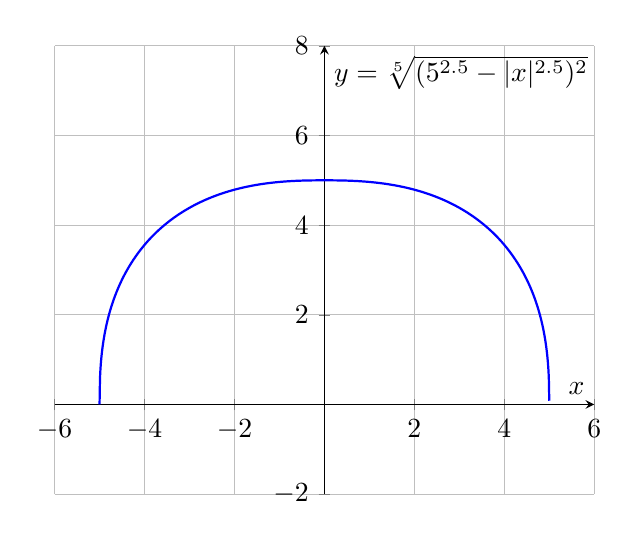
\begin{tikzpicture}
    \begin{axis}[
      xlabel=$x$,
      ylabel={$y=\sqrt[5]{(5^{2.5}-|x|^{2.5})^2}$},
      domain=-5:5,
      samples=1000,
      axis lines=middle,
      grid=both,
      xmin=-6,
      xmax=6,
      ymin=-2,
      ymax=8,
      enlarge x limits=false,
      enlarge y limits=false,
      ]
      \addplot+[mark=none,thick] {(5^(2.5)-abs(x)^(2.5))^(2/5)};
    \end{axis}
  \end{tikzpicture}
\end{center}

\subsection{Conclusión}
En resumen, la integración numérica es un método para aproximar el valor de una integral mediante el uso de fórmulas matemáticas y cálculos numéricos. Los métodos de integración numérica se utilizan cuando la integración analítica es difícil o imposible de realizar, o cuando la función a integrar es conocida solo a través de una tabla de valores o una gráfica.
\newline
Existen varios métodos de integración numérica, incluyendo la regla del trapecio, la regla de Simpson, y la regla de los puntos medios. Cada método tiene sus propias ventajas y desventajas, y la elección del método a utilizar dependerá del nivel de precisión deseado y la complejidad de la función a integrar.
\newline
Es importante destacar que la integración numérica es solo una aproximación del valor real de una integral, y la precisión de la aproximación dependerá del número de intervalos utilizados y de la fórmula numérica específica empleada. Por lo tanto, es importante tener en cuenta las limitaciones de la integración numérica y comprender cuándo es apropiado utilizarla.

\section{Problemario 5: 331-332}
\subsection{Problema 5}
Encunetre el area total acotada por la gráfica de la funcion dada y el eje en el intervalo dado.

\begin{center}
  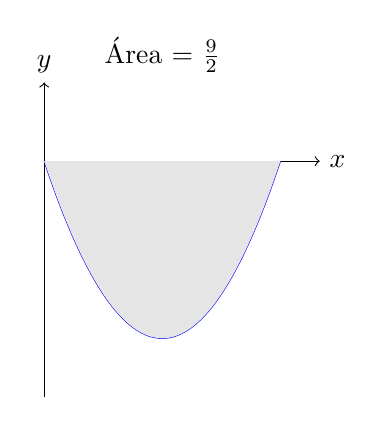
\begin{tikzpicture}
    \draw[->] (0,0) -- (3.5,0) node[right] {$x$};
    \draw[->] (0,-3) -- (0,1) node[above] {$y$};
    \draw[scale=1,domain=0:3,smooth,variable=\x,blue] plot ({\x},{\x*\x - 3*\x});
    \fill[gray!20,domain=0:3,smooth,variable=\x] (0,0) -- plot ({\x},{\x*\x - 3*\x}) -- (3,0) -- cycle;
    \draw (1.5,1) node[above] {Área = $\frac{9}{2}$};
  \end{tikzpicture}
\end{center}

Calculando el area:
\begin{align*}
  A = \int_{0}^{3} -(x^2-3x)dx = \left.\left(-\frac{1}{3}x^3-\frac{3}{2}x^2\right)\right|_{0}^{3} = \frac{9}{2} - 0 = \frac{9}{2}
\end{align*}

\subsection{Problema 17}
Encunetre el area total acotada por la gráfica de la funcion dada y el eje en el intervalo dado.
\begin{center}
  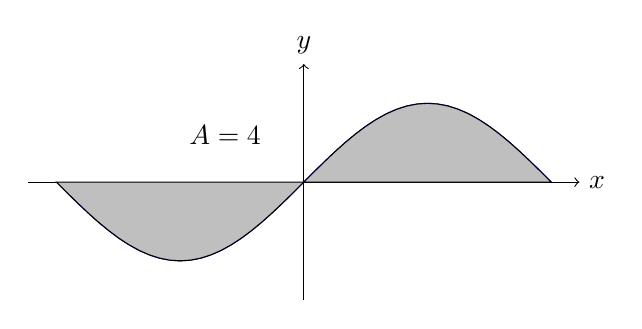
\begin{tikzpicture}
    \draw[->] (-3.5,0) -- (3.5,0) node[right] {$x$};
    \draw[->] (0,-1.5) -- (0,1.5) node[above] {$y$};
    \draw[scale=1,domain=-pi:pi,smooth,variable=\x,blue] plot ({\x},{sin(\x r)});
    \draw[fill=gray!50,domain=0:pi] (0,0) -- plot ({\x},{sin(\x r)}) -- (pi,0) -- cycle;
    \draw[fill=gray!50,domain=-pi:0] (0,0) -- plot ({\x},{sin(\x r)}) -- (-pi,0) -- cycle;
    \node at (-1,0.6) {$A=4$};
  \end{tikzpicture}
\end{center}

Integrando y evaluando:
\begin{align*}
  A = \int_{-\pi}^{0} -sin(x)dx +\int_{0}^{\pi} sin(x)dx = \dots \\ \dots = \left.cos(x)\right|_{-\pi}^{0} - \left.cos(x)\right|_{0}^{\pi} = [1-(-1)] - (-1-1) = 4
\end{align*}

\subsection{Problema 29}
Encuentre el area de ka region acotada por la grafica de las funciones dadas.

\begin{align*}
  y =
  \begin{cases}
    4(1-x^2) \\ 1-x^2
  \end{cases}
\end{align*}
Generando una grafica talque asi:
\begin{center}
  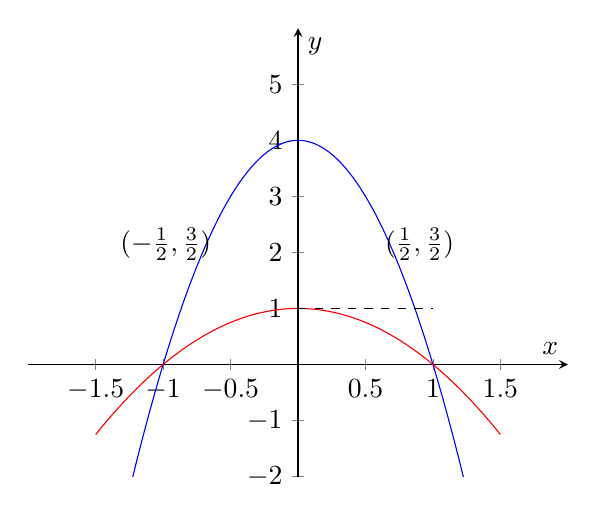
\begin{tikzpicture}
    \begin{axis}[
        axis lines=middle,
        xlabel=$x$,
        ylabel=$y$,
        xmin=-2, xmax=2,
        ymin=-2, ymax=6,
        xtick={-1.5,-1,-0.5,0.5,1,1.5},
        ytick={-2, -1, 0, 1, 2, 3, 4, 5},
        domain=-1.5:1.5,
        samples=100
      ]

      \addplot[blue, domain=-1.5:1.5] {4*(1-x^2)};
      \addplot[red, domain=-1.5:1.5] {1-x^2};
      \addplot[dashed, black] coordinates {(0,0) (0,4)};
      \addplot[dashed, black] coordinates {(0,1) (1,1)};

      \node[label={above right:$(\frac{1}{2},\frac{3}{2})$}] at (axis cs:0.5,1.5) {};
      \node[label={above left:$(-\frac{1}{2},\frac{3}{2})$}] at (axis cs:-0.5,1.5) {};

    \end{axis}
  \end{tikzpicture}
\end{center}

Integrando y evaluando:
\begin{align*}
  A = \int_{-1}^{1} (4(1-x^2)-(1-x^2))dx = \int_{-1}^{1} (3-3x^2)dx = \left.(3x-x^3)\right|_{-1}^{1} = 2-(-2) = 4
\end{align*}

\subsection{Problema 41}
Encuentre el area de ka region acotada por la grafica de las funciones dadas.

\begin{align*}
  x =
  \begin{cases}
    -y \\2-y^2
  \end{cases}
\end{align*}

Graficando:
\begin{center}
  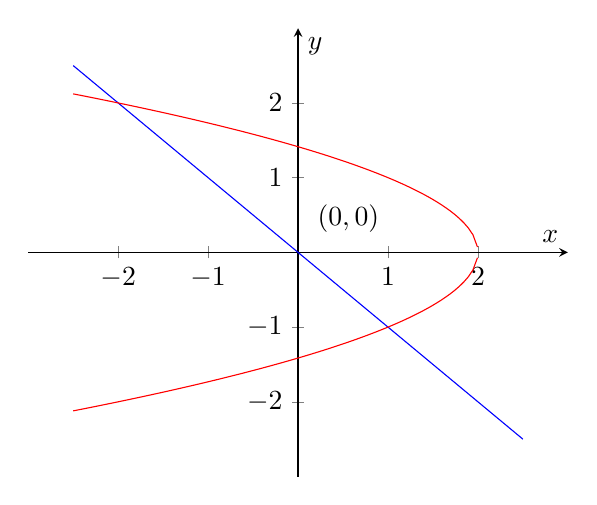
\begin{tikzpicture}
    \begin{axis}[
        axis lines=middle,
        xlabel=$x$,
        ylabel=$y$,
        xmin=-3, xmax=3,
        ymin=-3, ymax=3,
        xtick={-2, -1, 0, 1, 2},
        ytick={-2, -1, 0, 1, 2},
        domain=-3:3,
        samples=100
      ]

      \addplot[blue, domain=-2.5:2.5] {-x};
      \addplot[red, domain=-2.5:2.5] {sqrt(2-x)};
      \addplot[red, domain=-2.5:2.5] {-sqrt(2-x)};

      \node[label={above right:$(0,0)$}] at (axis cs:0,0) {};
    \end{axis}
  \end{tikzpicture}
\end{center}
Integrando y evaluando:
\begin{align*}
  A = \int_{-1}^{2} [(2-y^2)-(-y)]dy = \int_{-1}^{2} (2+y-y^2)dy = \dots \\ \dots = \left.\left(2y+\frac{1}{2}y^2 - \frac{1}{2}y^3\right)\right|_{-1}^{2} = \frac{10}{3} - \left(-\frac{7}{6}\right) = \frac{9}{2}
\end{align*}

\subsection{Problema 53}
Interprete la integral definida dada como el area de a region acotada por la grafica de dos funciones sobre un intervalo. Evalue y trace la region

\begin{align*}
  \int_{0}^{2}\left|\frac{3}{x+1}-4x\right|dx = \int_{0}^{\frac{1}{2}}\left[\frac{3}{x+1}-4x\right]dx + \int_{\frac{1}{2}}^{2} \left[-\frac{3}{x+1}+4x\right]dx = \dots \\ \dots = (3ln|x+1|-2x^2)_{0}^{\frac{1}{2}} + (3ln|x+1|-2x^2)_{\frac{1}{2}}^{2} =\dots \\ \dots = 3ln\frac{3}{2}-\frac{1}{2}+8-3ln3-\frac{1}{2}+3ln\frac{3}{2} = 7+3ln\frac{3}{4} \approx 6.1370
\end{align*}

\subsection{Problema 65}

\begin{wrapfigure}{r}{0.45\textwidth}
  \centering
  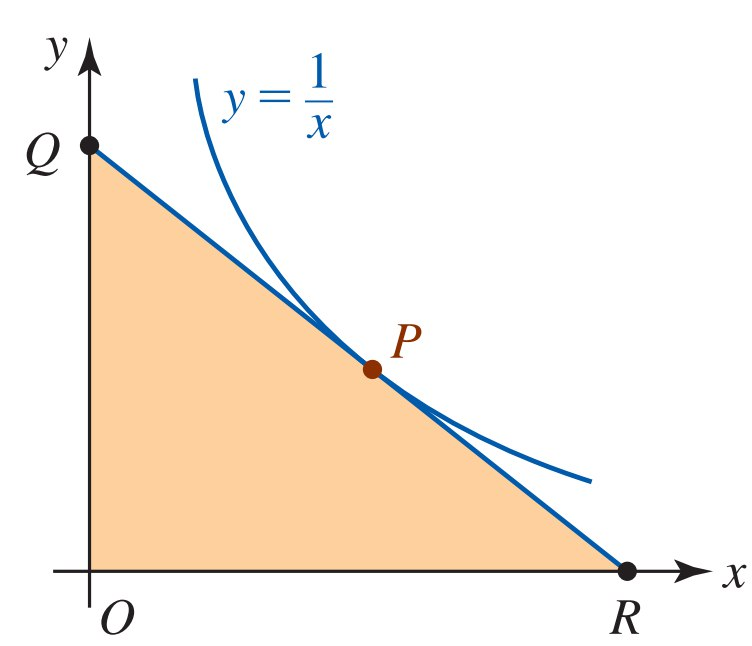
\includegraphics[width=0.37\textwidth]{./multimedia/Problema65.jpg}
\end{wrapfigure}
El segmento de recta entre $ Q$ y $R $ mostrado en la figura es tangente a la grafica de $ y =  \frac{1}{x} $ en el punto P. Demuestre que el area del triangulo $ QOR $ es independiente de las coordenadas de  $ P $.\newline
En P($ x_0$, $ 1/x_0$) la pendiente del segmento de línea es $ 1/x^2_0$. La ecuación de la recta a $ Q $ y $R$ es entonces $y =  x/x^2_0 + 2/x_0$. Estableciendo $ y = 0$ vemos que la inteseccion de $ x$ es $ 2x_0$. El área es

\begin{align*}
  \int_{0}^{2x_0}\left[-\frac{1}{x_0^2}x+\frac{2}{x_0}\right]dx = \left.\left(-\frac{1}{2x_0^2}x^2+\frac{2}{x_0}x\right)\right]_0^{2x_0} = -2+4 = 2,
\end{align*}
que no depende de $x_0$.

\subsection{Conclusión}
En conclusión, el cálculo del área bajo la curva es un concepto fundamental en el campo de las matemáticas, con diversas aplicaciones en distintas áreas de la ciencia y la ingeniería. Algunas de las aplicaciones más comunes son en el cálculo de integrales, la física, la economía y finanzas, y la ingeniería. El área bajo la curva se utiliza para calcular la longitud de arcos, el volumen de sólidos, el trabajo realizado por una fuerza en un desplazamiento, la energía cinética y potencial, el costo total, la ganancia total o la utilidad total, y puede utilizarse para la optimización de la producción o la maximización de la ganancia, entre otras aplicaciones. El cálculo del área bajo la curva es un concepto fundamental que permite entender y modelar de manera más precisa el comportamiento de diversas variables en distintos campos de la ciencia y la ingeniería.

\section{Problemario 6: 344-345}
\subsection{Problema 5}
\begin{wrapfigure}{l}{0.45\textwidth}
  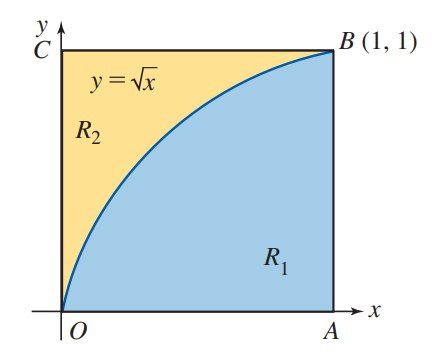
\includegraphics[width=0.4\textwidth]{multimedia/Problema5.jpeg}
\end{wrapfigure}
Use el metodo de los cascarones para enontrar el volumen del solido de revolucion que se forma al girar la region dada alrededor de la recta indicada.
El giro se dara alrededor de $ AB $ con el area $R_1$

\begin{align*}
  V = 2\pi\int_{0}^{1} (1-x)\sqrt{x}dx =\dots \\ \dots = 2\pi\left.\left(\frac{2}{\pi}x^{\frac{3}{2}}-\frac{2}{3}x^{\frac{5}{2}}\right)\right|_0^1 =\dots \\ \dots = \frac{8\pi}{15}
\end{align*}
\newline
\newline
\subsection{Problema 17}
Use el metodo de cascarones para encontrar el volumen del solido de revolucion que se forma al girar la region acotada por las graficas de las ecuaciones dadas alrededor de a recta o eje que se indica.
Siendo las ecuaciones las siguientes:
\begin{align*}
  y=x^{\frac{1}{3}},x=1,y=0;y=-1
\end{align*}
\begin{center}
  \begin{tikzpicture}[scale=1.5]
    \draw[->] (-0.5,0) -- (1.5,0) node[right] {$x$};
    \draw[->] (0,-1.5) -- (0,1.5) node[above] {$y$};
    \draw[domain=0:1,smooth,variable=\x,blue] plot ({\x},{\x^(1/3)});
    \draw[dashed] (1,-1.3) -- (1,1.5) node[above] {$x=1$};
    \draw[dashed] (-0.5,0) -- (1.5,0) node[right] {$y=0$};
    \draw[dashed] (-0.5,-1) -- (1.5,-1) node[right] {$y=-1$};
  \end{tikzpicture}
\end{center}
Solucionando:
\begin{align*}
  V = 2\pi\int_{0}^{1}(y+1)(1-y^3)dy =2\pi \int_{0}^{1}(1+y-y^3-y^4)dy = \dots \\ \dots = 2\pi\left.\left(y+\frac{1}{2}y^2-\frac{1}{4}y^4-\frac{1}{5}y^5\right)\right|_0^1 = \frac{21\pi}{10}
\end{align*}

\subsection{Problema 29}
Use el metodo de cascarones para encontrar el volumen del solido de revolucion que se forma al girar la region acotada por las graficas de las ecuaciones dadas alrededor de a recta o eje que se indica.
Siendo las ecuaciones las siguientes:
\begin{align*}
  y = sin (x^2) , x = 0, y = 1; y
\end{align*}

\begin{center}
  \begin{tikzpicture}[scale=1.5]
    \draw[->] (-0.5,0) -- (1.8,0) node[right] {$x$};
    \draw[->] (0,-1.2) -- (0,1.2) node[above] {$y$};
    \draw[domain=0:sqrt(pi/2),smooth,variable=\x,blue] plot ({\x},{sin(deg(\x^2))});
    \draw[dashed] (0,-1) -- (1.8,-1) node[right] {$y=-1$};
    \draw[dashed] (0,1) -- (1.8,1) node[right] {$y=1$};
    \draw[dashed] (1.25331413732,0) -- (1.25331413732,1.2) node[above] {$x=\sqrt{\pi/2}$};
  \end{tikzpicture}
\end{center}

Solucionando:
\begin{align*}
  V = 2\pi\int_{0}^{\sqrt{\frac{\pi}{2}}}(x-xsin(x^2))dx = 2\pi\left.\left(\frac{1}{2}x^2+\frac{1}{2}cos(x^2)\right)\right|_0^{\sqrt{\frac{\pi}{2}}} = \dots \\ \dots = 2\pi\left(\frac{\pi}{4}-\frac{1}{2}\right)=\frac{\pi^2-2\pi}{2}
\end{align*}

\subsection{Conclusión}
La integración por el método de cascarones es una técnica que se utiliza para calcular el volumen de sólidos de revolución. La idea básica del método es descomponer el sólido en una serie de cascarones cilíndricos concéntricos de espesor infinitesimal. Luego se integra el área de cada cascarón a lo largo del eje de rotación para obtener el volumen total del sólido.\\
En resumen, el método de cascarones es una herramienta útil para calcular el volumen de sólidos de revolución en casos en los que la integración directa es difícil o imposible.

\section{Problemario 7}
\subsection{Problema 5}
La base de un sólido es un triángulo isósceles cuya base y altura miden, respectivamente, 4 y 5 pies. Las secciones transversales perpendiculares a la altura son semicírculos. Encuentre el volumen del sólido.
\begin{align*}
  y = -\frac{2}{5}x+2 &  & A(x) = \frac{1}{2}\pi y^2 = \frac{2\pi}{25}(x-5)^2
\end{align*}
\begin{align*}
  V= \int_{0}^{5} \left(\frac{2\pi}{25}(x-5)^2 \right)dx = \left.\frac{2\pi}{75}(x-5)^2 \right|_0^5 =\frac{10\pi}{3}ft^3
\end{align*}

\subsection{Problema 17}
Use el metodo de arandelas para encontrar el volumen del solido de revolucion que se forma al girar la region acotada por las ecuaciones dadas alrededor de la recta o eje que se indica.
El sistema es:
\begin{align*}
  y = \frac{1}{x}, x = \frac{1}{2},y = \frac{1}{2} ; y
\end{align*}
\begin{center}
  \begin{tikzpicture}[scale=2]
    \draw[<->] (-0.2,0) -- (2.2,0) node[right] {$x$};
    \draw[<->] (0,-0.2) -- (0,2.2) node[above] {$y$};
    \draw[domain=0.5:1.8,smooth,variable=\x,blue] plot ({\x},{1/\x});
    \draw[dashed] (0.5,0.5) -- (0.5,2);
    \draw[dashed] (0.5,0.5) -- (2,0.5);
    \filldraw[black] (0.5,0.5) circle (0.02) node[anchor=south west] {$(\frac{1}{2},\frac{1}{2})$};
  \end{tikzpicture}
\end{center}
\begin{align*}
  V = \pi \int_{\frac{1}{2}}^{1}\left[\left(\frac{1}{y}\right)^2-1^2\right]dy = \pi\int_{\frac{1}{2}}^{1}(y^{-2}-1)dy = \dots \\ \dots = \pi\left.\left(-\frac{1}{y}-y\right)\right|_{\frac{1}{2}}^1 = \pi \left[-2-\left(-\frac{5}{2}\right)\right] = \frac{\pi}{2}
\end{align*}
\section{Problema 29}
Use el metodo de arandelas para encontrar el volumen del solido de revolucion que se forma al girar la region acotada por las ecuaciones dadas alrededor de la recta o eje que se indica.
El sistema es:
\begin{align*}
  x^2-y^2=16,x=5;y
\end{align*}

\begin{center}
  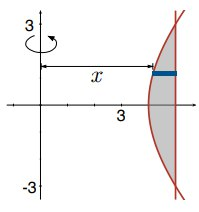
\includegraphics[width=0.3\textwidth]{multimedia/photo_5030828484276103944_m.jpg}
\end{center}
\begin{align*}
  V=\pi\int_{-3}^{3}\left[5^2-\left(\sqrt{y^2+16}\right)^2\right]dy = \int_{-3}^{3}(9-y^2)dy = \dots \\ \dots = \pi\left.\left(9y-\frac{1}{3}y^3\right)\right|_{-3}^3 = \pi[18-(-18)] = 36\pi
\end{align*}
\subsection{Conclusión}
La integración por arandelas es una técnica de cálculo integral que se utiliza para encontrar el volumen de un sólido de revolución generado al girar una región plana alrededor de un eje. En este método, se divide el sólido en infinitas arandelas y se calcula el volumen de cada una de ellas.
Para calcular el volumen de una arandela, se utiliza la fórmula:
\newline
$$V = \pi \int_{a}^{b} (R(x)^2 - r(x)^2) dx$$
\newline
Donde $R(x)$ es el radio exterior de la arandela y $r(x)$ es el radio interior. El intervalo de integración $[a,b]$ corresponde a la región plana girada alrededor del eje.
\newline
La integración por arandelas es una técnica muy útil y versátil para calcular el volumen de sólidos de revolución.
\section{Problemario 8: 347-348}
\subsection{Problema 5}
Encuentre la longitud de la grafica de la funcion dada sobre el intervalo indicado.
\begin{align*}
  y = \frac{2}{3}(x^2+1)^{\frac{3}{2}}; [1,4]
\end{align*}
Resolviendo:
\begin{align*}
  y'=2x(x^2+1)^{\frac{1}{2}}\\ s =\int_{1}^{4}\sqrt{1+4x^2(x^2+1)}dx = \int_{1}^{4}(2x^2+1)dx = \dots \\ \dots = \left.\left(\frac{2}{3}x^3+x\right)\right|_1^4=\frac{140}{3}-\frac{5}{3} = 45
\end{align*}

\subsection{Problema 17}
Use:
$$
L=\int_{c}^{d}\sqrt{1+\left(\frac{dx}{dy}^2\right)}dy
$$
Para encontrar la longitud de la grafica de la ecuacion dada sobre el intervalo indicado.
Siendo la ecuacion:
$$
x = 4-y^{\frac{2}{3}};[0,8s]
$$
Resolviendo:
\begin{align*}
  \frac{dx}{dy}=-\frac{2}{3}y^{-1/3}\\ s = \int_{0}^{8}\sqrt{1+\frac{4}{9}y^{-\frac{2}{3}}}dy = \frac{1}{3}\int_{0}^{8}y^{-\frac{1}{3}}\sqrt{9y^{\frac{2}{3}}+4}dy = \dots \\ u =9y^{\frac{2}{3}}+4, du =6y^{-\frac{1}{3}}dy \\ \frac{1}{18}\int_{4}^{40}u^{\frac{1}{2}} du = \left.\frac{1}{27}u^{-\frac{3}{2}}\right|_4^{40} = \frac{1}{27}(40^{\frac{3}{2}}-8)\approx 9.0734
\end{align*}
\subsection{Conclusión}
La longitud de una curva es un concepto matemático que se refiere a la distancia total recorrida por la curva. La longitud de una curva puede ser calculada utilizando técnicas de cálculo integral, tales como la integral de longitud de arco.
\\
La integral de longitud de arco es una herramienta matemática utilizada para calcular la longitud de una curva en el plano. Esta técnica se basa en la idea de aproximar la curva con pequeños segmentos rectos y sumar las longitudes de estos segmentos para obtener una aproximación de la longitud total de la curva. Al hacer que los segmentos rectos sean cada vez más pequeños, la aproximación se hace más precisa.
\\
En resumen, la longitud de una curva puede ser calculada utilizando la integral de longitud de arco, la cual es una técnica de cálculo integral que se basa en la aproximación de la curva con pequeños segmentos rectos.

\section{Problemario 10}
\subsection{Problema 3}
Determine el area de la superficie de aquella porcion del cilindro $x^2+z^2=16$ que esta sobre la region en el primer cuadrante acotada por las graficas de $x=0, x=2, y=0,y=5$.
Usando $f(x,y)=z=\sqrt{16-x^2}$ podemos observar que para $0\leq x\leq2$ and $0\leq y\leq5$. Por lo tanto la superficie esta completamente por encima de la region. Ahora $f_x = - \frac{x}{\sqrt{16-x^2}}, f_y = 0, 1+f_x^2+f_y^2 = 1+\frac{x^2}{16-x^2}=\frac{16}{16-x^2}$  y 
\begin{align*}
  A =\int_{0}^{5}\int_{0}^{2}\frac{4}{\sqrt{16-x^2}}dxdy = \left.4 \int_{0}^{5}sin^{-1}(\frac{x}{4})\right|_0^2dy=4\int_{0}^{5}\frac{\pi}{6}dy=\frac{10\pi}{3}
\end{align*}
\subsection{Conclusión}
En conclusión, el cálculo del área de la superficie de un sólido de revolución por el método de discos o arandelas consiste en descomponer el sólido en una serie de discos o anillos con espesor infinitesimal y calcular el área de cada uno de ellos. Luego, se integra el área de cada disco o anillo a lo largo del eje de revolución para obtener el área total de la superficie. Este método es útil en aplicaciones como la construcción de tanques de almacenamiento, la fabricación de piezas de maquinaria y la modelación de objetos tridimensionales en la ingeniería y el diseño.
\end{document}
